%!TEX root = /Users/ego/Boulot/TKZ/tkz-euclide/doc_fr/TKZdoc-euclide-main.tex

\section{Les arcs} 

\begin{NewMacroBox}{tkzDrawArc}{\oarg{local options}\parg{O,\dots}\parg{\dots} }

 \emph{Cette macro trace un arc de centre O. Suivant les options, les arguments diffèrent.   Il s'agit de déterminer un point de départ et un point d'arrivée. Soit le point de départ est donné, c'est ce qu'il y a de plus simple, soit on donne le rayon de l'arc. Dans ce dernier cas, il est nécessaire d'avoir deux angles. On peut soit donner directement les angles, soit donner des nodes qui associés au centre permettront de les déterminer.}   
  

\medskip

\begin{tabular}{lll}
\toprule
options             & défaut & définition                         \\ 
\midrule
\TOline{towards}{towards}{O est le centre et l'arc par de A vers (OB)} 
\TOline{rotate} {towards}{l'arc part de A et l'angle détermine sa longueur } 
\TOline{R}{towards}{On donne le rayon et deux angles} 
\TOline{R with nodes}{towards}{On donne le rayon et deux points}
\TOline{delta}{0}{angle ajouté de chaque côté } 
\bottomrule
\end{tabular}

\medskip
\emph{Il faut ajouter bien sûr tous les styles de \TIKZ pour les tracés}

\medskip

\begin{tabular}{lll}
\toprule
options             & arguments & exemple                         \\ 
\midrule
\TOline{towards}{\parg{pt,pt}\parg{pt}}{\tkzcname{tkzDrawArc[delta=10](O,A)(B)}} 
\TOline{rotate} {\parg{pt,pt}\parg{an}}{\tkzcname{tkzDrawArc[rotate,color=red](O,A)(90)}}
\TOline{R}{\parg{pt,$r$}\parg{an,an}}{\tkzcname{tkzDrawArc[R,color=blue](O,2 cm)(30,90)}}
\TOline{R with nodes}{\parg{pt,$r$}\parg{pt,pt}}{\tkzcname{tkzDrawArc[R with nodes](O,2 cm)(A,B)}}
\bottomrule
\end{tabular}
\end{NewMacroBox}

Quelques exemples : 

\subsection{\tkzcname{tkzDrawArc} et \tkzname{towards}}
Il est inutile de mettre \tkzname{towards}. Dans ce premier exemple l'arc part de A et va sur B. L'arc qui va de B vers A est différent. On obtient le saillant en allant dans le sens direct du cercle trigonométrique.
\begin{tkzexample}[latex=6cm]
\begin{tikzpicture}
  \tkzDefPoint(0,0){O}
  \tkzDefPoint(2,-1){A}
  \tkzDefPointBy[rotation= center O angle 90](A)
  \tkzGetPoint{B}
  \tkzDrawArc[color=blue](O,A)(B) 
  \tkzDrawArc(O,B)(A)
  \tkzDrawLines[add = 0 and .5](O,A O,B)
  \tkzDrawPoints(O,A,B)
  \tkzLabelPoints[below](O,A,B)  
\end{tikzpicture}
\end{tkzexample}


\subsection{\tkzcname{tkzDrawArc} et \tkzname{towards}}
Dans celui-ci, l'arc part de A mais s'arrête sur la droite (OB).
 
\begin{tkzexample}[latex=6cm]
\begin{tikzpicture}[scale=1.5] 
  \tkzDefPoint(0,0){O}
  \tkzDefPoint(2,-1){A}
  \tkzDefPoint(1,1){B} 
  \tkzDrawArc[color=blue](O,A)(B)
  \tkzDrawArc[color=Maroon](O,B)(A)
  \tkzDrawArc(O,B)(A)
  \tkzDrawLines[add = 0 and .5](O,A O,B) 
  \tkzDrawPoints(O,A,B)
  \tkzLabelPoints[below](O,A,B)  
\end{tikzpicture}
\end{tkzexample}

\subsection{\tkzcname{tkzDrawArc} et \tkzname{rotate}}
\begin{tkzexample}[latex=5cm] 
\begin{tikzpicture} 
  \tkzDefPoint(0,0){O}
  \tkzDefPoint(2,-2){A}
  \tkzDefPoint(60:2){B}
  \tkzDrawLines[add = 0 and .5](O,A O,B)
  \tkzDrawArc[rotate,color=red](O,A)(180)
  \tkzDrawPoints(O,A,B)
  \tkzLabelPoints[below](O,A,B) 
\end{tikzpicture}
\end{tkzexample} 


\subsection{\tkzcname{tkzDrawArc} et \tkzname{R}} 
\begin{tkzexample}[latex=5cm]   
\begin{tikzpicture}
  \tkzDefPoints{0/0/O}
  \tikzset{compass style/.append style={<->}}   
  \tkzDrawArc[R, color=orange,double](O,3cm)(270,360)
  \tkzDrawArc[R, color=blue,double](O,2cm)(0,270) 
  \tkzDrawPoint(O)
  \tkzLabelPoint[below](O){$O$}  
\end{tikzpicture} 
\end{tkzexample}

\subsection{\tkzcname{tkzDrawArc} et \tkzname{R with nodes}} 
\begin{tkzexample}[latex=5cm]
\begin{tikzpicture}
  \tkzDefPoint(0,0){O}
  \tkzDefPoint(2,-1){A}
  \tkzDefPoint(1,1){B}
  \tkzCalcLength(B,A)\tkzGetLength{radius}
  \tkzDrawArc[R with nodes](B,\radius pt)(A,O)
\end{tikzpicture}
\end{tkzexample}

\subsection{\tkzcname{tkzDrawArc} et \tkzname{delta}}
Cette option permet un peu comme \tkzcname{tkzCompass} de placer un arc et de déborder de chaque côté. delta est une mesure en degré.

\begin{tkzexample}[latex=7cm] 
\begin{tikzpicture} 
 \tkzInit
 \tkzDefPoint(0,0){A}
 \tkzDefPoint(5,0){B}
 \tkzDefPointBy[rotation= center A%
                angle 60](B) \tkzGetPoint{C} 
 \tkzSetUpLine[color=gray]
 \tkzDefPointBy[symmetry= center C](A)
    \tkzGetPoint{D} 
 \tkzDrawSegments(A,B A,D)
 \tkzDrawLine(B,D)
 \tkzSetUpCompass[color=orange]
 \tkzDrawArc[delta=10](A,B)(C)
 \tkzDrawArc[delta=10](B,C)(A)
 \tkzDrawArc[delta=10](C,D)(D)
 \tkzDrawPoints(A,B,C,D)
 \tkzLabelPoints(A,B,C,D)
 \tkzMarkRightAngle(D,B,A)
\end{tikzpicture}
\end{tkzexample} 


 \endinput
 
